\documentclass[12pt,a4j,twocolumn]{jarticle}

\usepackage[dvipdfmx]{graphicx}

\textheight=24cm \textwidth=16.5cm
\oddsidemargin=-8pt \topmargin=-25pt

\title{Ich besuchte David Hilbert}
\author{Autor: Teiji Takagi,\quad Publikation: November 1932\thanks{https://bit.ly/3Oeyrlg}\\
\"Ubersetzer: Takahiro Nakamura
}
\date{}

\begin{document}

\maketitle

\noindent
Ich besuchte David Hilbert in G\"ottingen am 8 Oktober 1932.

Am Abend um 7:15 Uhr oder fr\"uher, wanderte ich hin und her, durch den Weg 
vor dem 29sten Haus an der Wilhelm-Weber-Stra\ss e.
Da sah ich manche Sterne, die man k\"urzlich selten sehen kann.
Der herbstliche Wind war so kalt.
Es entsprach meiner Stimmung,
dass einige gefallene Bl\"atter von einer Linde verstreut waren.

Dann hatte ich ein Rendezvous mit einem Fr\"aulein.
Das Fr\"aulein war Professorin Emmy Noether.
Sie hatte mir freundlicherweise versprochen, 
dass wir zusammen Professor Hilbert besuchen w\"urden.
Sie sagte, wenn ich ihn f\"ur mich besuchte,
w\"urde ich um stockendes Gespr\"ach verlegen sein.

Das Haus des Professors ist 29st an der Wilhelm-Weber-Stra\ss e.
Es ist schon lange her, dass ich sein Haus erstmals besuchte.
Damals am Haus war ein allgemeines Pf\"ortchen, und ein kleiner Vorgarten mit Pflanzen.
Aber die Pflanzen wurden ein W\"aldchen in drei\ss ig Jahren.
Wegen der Dunkelheit, konnte ich nicht erkennen, 
ob es Pflaumen oder Birnen im W\"aldchen gab.
Jedenfalls die Saison war gerade richtig f\"ur Obst.
Ich dachte mir, dass er und seine Frau sicher die Obst auf ihrem Tisch h\"auften.
Der Flur war auch dunkel. Da kam eine Haush\"alterin heraus, um anzumelden.
Aber Professorin N, die das Haus gut kannte, verlie\ss\ die Haush\"alterin,
und leitete mich schnell ins G\"astezimmer, ohne uns angemeldet zu haben.
Vielleicht hatte sie schon telefonisch angemeldet.
Professor H kam bald heraus, und sagte: ``Ich wei\ss\ euer Versprechen.
Herzlich willkommen." Dieses Jahr ist Professor H genau siebzig Jahre alt.
Er sah gesund aus, und zeigte ein L\"acheln auf dem knabenhaften Gesicht wie fr\"uher.
Mehrere Jahre vorher, bekam er eine Krankheit, die schwer zu heilen war.
Ich h\"orte, die Krankheit hei\ss e so und so auf Latein, das ich verga\ss.
Seine Leber soll nicht richtig funktioniert haben.
Einmal hatte er die Hoffnung der Heilung fast aufgegeben.
Dann gerade in Amerika wurde eine neue Arznei entdeckt.
Die Arznei soll sein Leben eben noch gerettet haben.
Aber es war unsicher, ob die blo\ss e Arznei genug wirksam war.
Deshalb soll er ein Viertel roher Leberwurst t\"aglich essen.
Er sagte, wenn er diese Kur aufh\"orte,
w\"urde sein Leben jede Woche schwinden, wegen der unheilbaren Krankheit.
Die Kur wirkte gut, und er bekam die Lebenskraft wieder.
Damit konnte er dieses Jahr zum Kongress in Z\"urich ausgehen.

Vorletztes Jahr nahm Professor H seinen Abschied von der Universit\"at G\"ottingen.
Danach soll er jede Woche einmal eine Vorlesung in der Uni noch frei halten.
Vielleicht liest er \"uber die Grundlagen der Mathematik vor.
``In diesem Wintersemester wollte ich alles tun, was ich noch nicht erledigt habe.
Aber wider Erwarten sind Assistenzprofessoren kritisch gegen meine Studien.
Ich kann doch nichts anders tun als langsam zu studieren, ohne mich zu treiben.
Formalismus ist sehr wichtig f\"ur Mathematik.
Das muss jeder von uns bejahen.
Aber manchmal kann man mit dem Formalismus nicht alles erledigen.
Da gibt es viele Probleme..." murmelte der alte Professor,
als ob er mit sich selbst spr\"ache.
Dabei konnte ich nicht umhin, heimliche Tr\"anen zu weinen.

Einige Jahre vorher, schrieb ich eine popul\"are
Erkl\"arung \"uber die Grundlagen der Mathematik.
Darin ist ein Satz des folgenden Inhalts:
``Professor H will jeden Kuckuck rufen lassen, um seine lebenslange Erinnerung zu machen."
Damit dr\"uckte ich freilich aus, wie eifrig er die Grundlagen der Mathematik l\"osen will.
Aber die Allegorie vom Kuckuck war unzutreffend.
Es war zu bef\"urchten, dass der Satz einen h\"ohnischen Eindruck auf die Leser machte.
Deshalb wollte ich woanders die folgende Bedeutung beschreiben:
``Die Grundlagen der Mathematik m\"ogen vollendet werden. 
Oder sie m\"ogen unvollendet werden.
Immerhin w\"unsche ich nur, dass Professor H seine letzten Jahre in Behagen verbringt."
Jetzt ist es mir eingefallen, dass ich das zu beschreiben verga\ss.
Trotz des Kampfs mit der unheilbaren Krankheit,
und trotz mancher krittelei von j\"ungeren Assistenzprofessoren,
muss er das Gesetz der ausgeschlossenen Mitte beweisen. Warum?
Es kommt ihm gar nicht in Frage, den Rest des Lebens zu genie\ss en.
Es scheint als ob er in H\"ollenqualen lebte, oder?
Furchtbar ist der Wissensdrang, der auch unheilbar ist.

Dann schaute ich auf Professorin N. Offenbar sah sie auch verlegen aus.
Vermutlich h\"orte sie ihn fast jeden Tag murmeln.
Es war ganz nat\"urlich, dass sie anderes Gef\"uhl als ich hatte,
denn ich traf ihn nach zehn Jahren.

Professor H lenkte oft das Gespr\"ach in verschiedene Richtungen.
Er redete sogar \"uber soziale Fragen.
Er sagte, es gebe allzu viele Menschen, die Erde sei zu eng,
aber der Fortschritt der Wissenschaft w\"urde die Schwierigkeiten irgendwie \"uberwinden,
und so weiter. Wenn ich mich nicht t\"ausche, sagte er auch:
``Ach was, Russki k\"onnen nichts tun."

Allm\"ahlich wurde das Gespr\"ach transzendental.
``Ich glaube fest an unendlichen Fortschritt der Menschheit.
Die f\"unf tausend Jahre lange Geschichte der Menschheit ist \"uberhaupt
Null im Vergleich zur Unendlichkeit der Zeit.
Inzwischen sind wir jedoch bisher weit fortgeschritten.
Au\ss erdem erkl\"art die Naturwissenschaft, dass  wir uns in Milliarden Jahren 
von Sch\"aumen zur heutigen Menschheit entwickelt haben.
Sowohl Milliarde wie Billion sollen wenig sein.
Hiernach werden wir in ewigen Zeiten unendlich fortschreiten..."

Als ein Steinblock seit Milliarde Jahren erschien,
winkte Professorin N mir mit den Augen.
W\"ahrend des ewigen Fortschrittes standen wir auf.
``Wir sind unwillk\"urlich lange geblieben, denn wir haben
deiner interessanten Rede zugeh\"ort. Du magst doch wohl schon m\"ude sein. 
Herzlichen Dank. Angenehme Ruhe."

Nachher am Abend h\"orte ich Herrn C sagen, 
die Rede der Milliarde Jahre sei bekannt heutzutage in der Uni.
Darin soll man oft sagen: ``Du hast ebenfalls die Milliarde geh\"ort."
Ich h\"orte, Professor H lese neulich gern {\it Die Weltgeschichte} von H. G. Wells
(ein bekanntes Buch, neulich \"ubersetzt ins Deutsche).

Professor H mag das Buch von Wells lesen,
oder mag er \"uber den Fortschritt der Menschheit in Milliarde Jahren nachdenken,
als er eine Pause nach seinem mathematischen Studium macht.
Das ist mir gut, wenn er Pausen macht. Dann macht es nichts, 
dass die J\"ungeren sich mit dem Ger\"ucht von der Milliarde unterhalten.
Zun\"achst ist das gut und gl\"ucklich.

Hier und da h\"orte ich Anekdoten \"uber Professor H:

\bigskip\noindent
An einem Abend lud Professor H G\"aste zum Haus ein.
Als die Ankunftszeit der G\"aste nahte, sah seine Frau K\"athe zuf\"allig seine Kleidung. 
Sie sagte: ``O, David, du musst deine Krawatte schnell wechseln, schnell,"
und lie\ss\ ihn zum ersten Stock hinaufgehen.
Inzwischen alle G\"aste sammelten sich im Haus.
Aber Professor H kam nicht herunter, obwohl die G\"aste auf ihn lange warteten.
Als sie die Haush\"alterin ihn holen lie\ss, schlief er im Bett ruhig ein...
(Herr A nennt diesen Fall die Analytische Fortsetzung von der L\"osung der Krawatte.)

\centerline{\begin{tabular}{c}\parbox{60mm}{\hfill}\\\hline\end{tabular}}

\bigskip\noindent
Bei seiner Vorlesung an einem Montag, soll ein Student gemerkt haben,
dass Professor H ein Loch in seiner Hose hatte.
Noch am Dienstag sah die Studenten das Loch.
Sie beobachteten keine Ver\"anderung des Lochs am Mittwoch, Donnerstag, und Freitag.
Daher wurde das Loch in der Hose des Professors bekannt in der Uni.
Dann berieten sich die Studenten. Sie beschlossen, ihm das Loch zu berichten,
ohne Kanten zu machen.
An einem Tag der n\"achsten Woche, spazierte Professor H mit den Studenten 
nach der \"Ubung des Seminars.
Dabei stie\ss\ er sich zuf\"allig an einem Rad eines Lastwagens.
Ein Student ergriff die Gelegenheit, und sagte:
``Vorsicht! Ei, Professors Hose ist verletzt worden."
Professor H sagte: ``Was? Wo? Ah, dieses Loch soll ich seit dem
letzten Semester haben."

\centerline{\begin{tabular}{c}\parbox{60mm}{\hfill}\\\hline\end{tabular}}

\bigskip\noindent
Noch eine Anekdote. Dies ist kurz, aber typisch Professor H.
Eines Tages besuchte ein Gast ihn zu Hause.
Der Besuch soll irgendwie eckig gewesen sein.
Der Gast und der Herr setzten sich, und sprachen einige Minuten miteinander,
\"uber gutes Befinden oder schlechtes Wetter.
Dann stand Professer H pl\"otzlich auf.
Er sah sich nach seiner Frau um, und sagte: ``He, K\"athe,
ich habe den Gast lange aufgehalten. Also wollen wir uns eine Mu\ss e geben..."

\vfill
\noindent
\parbox[t]{38mm}{
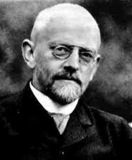
\includegraphics[width=38mm,bb=0 0 132 160]{Hilbert.jpg}\\
\centerline{David Hilbert}}\hfill
%
\parbox[t]{40mm}{
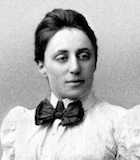
\includegraphics[width=40mm,bb=0 0 140 160]{Noether.jpg}\\
\centerline{Emmy Noether}}\\

\end{document}